\section{Signale}
\subsection{Harmonische Schwingungen}
Als harmonische Schwingung bezeichnet man eine sinusförmige Schwingung. 
\begin{equation*}
x(t) \underbrace{A}_{Amplitude} \cdot \sin(\underbrace{\omega}_{Kreisfrequenz}t +\underbrace{\phi}_{Phasenverschiebung})+\underbrace{c}_{DC-Anteil}
\end{equation*}
\begin{tabular}{|l|l|l|}
	\hline
	\textbf{Ordnung n}& \textbf{Frequenz}& \textbf{Name der Komponente}\\
	\hline $0$& $0$& Gleichstromanteil\\
	\hline $1$& $f_0$& Grundwelle / 1.Harmonische\\
	\hline $2$& $2f_0$& 1.Oberwelle / 2.Harmonische\\
	\hline $3$& $3f_0$& 2.Oberwelle/ 3.Harmonische\\
	\hline $n$& $nf_0$& n-1.Oberwelle / n-te .Harmonische\\
	\hline
\end{tabular}
\clearpage
\pagebreak
%TODO Fehler font beheben
\subsection{Logarithmische Darstellungen}
\renewcommand{\arraystretch}{1.2}
\begin{tabular}{ll}
	\parbox{7cm}{
		\scriptsize
		\begin{tabular}{|c|c|c|c|}
			\hline
			\textbf{Lrel. (dB)} & \textbf{Lrel. (NP)} & \textbf{P2/P1} & \textbf{A2/A1} \\ \hline
			$100.000$ & $11.513$ & $10^{10}$ & $10^5$ \\ \hline
			$90.000$ & $10.362$ & $10^9$ & $31622.777$ \\ \hline
			$80.000$ & $9.210$ & $10^8$ & $10^4$ \\ \hline
			$70.000$ & $8.059$ & $10^7$ & $3162.278$ \\ \hline
			$60.000$ & $6.908$ & $10^6$ & $10^3$ \\ \hline
			$50.000$ & $5.756$ & $10^5$ & $316.228$ \\ \hline
			$40.000$ & $4.605$ & $10^4$ & $10^2$ \\ \hline
			$30.000$ & $3.454$ & $10^3$ & $31.623$ \\ \hline
			\textbf{$20.000$} & $2.303$ & \textbf{$10^2$} & \textbf{$10.000$} \\ \hline
			$19.085$ & $2.197$ & $81.000$ & $9.000$ \\ \hline
			$19.000$ & $2.187$ & $79.433$ & $8.913$ \\ \hline
			$18.062$ & $2.079$ & $64.000$ & $8.000$ \\ \hline
			$18.000$ & $2.072$ & $63.096$ & $7.943$ \\ \hline
			$17.000$ & $1.957$ & $50.119$ & $7.079$ \\ \hline
			$16.902$ & $1.946$ & $49.000$ & $7.000$ \\ \hline
			$16.000$ & $1.842$ & $39.811$ & $6.310$ \\ \hline
			$15.563$ & $1.792$ & $36.000$ & $6.000$ \\ \hline
			$15.000$ & $1.727$ & $31.623$ & $5.623$ \\ \hline
			$14.000$ & $1.612$ & $25.119$ & $5.012$ \\ \hline
			\textbf{$13.979$} & $1.609$ & \textbf{$25.000$} & \textbf{$5.000$} \\ \hline
			$13.000$ & $1.497$ & $19.953$ & $4.467$ \\ \hline
			\textbf{$12.041$} & $1.386$ & \textbf{$16.000$} & \textbf{$4.000$} \\ \hline
			\textbf{$12.000$} & $1.382$ & $15.849$ & $3.981$ \\ \hline
			$11.000$ & $1.266$ & $12.589$ & $3.548$ \\ \hline
			\textbf{$10.000$} & $1.151$ & \textbf{$10.000$} & $3.162$ \\ \hline
			$9.542$ & $1.099$ & $9.000$ & $3.000$ \\ \hline
			$9.000$ & $1.036$ & $7.943$ & $2.818$ \\ \hline
			$8.000$ & $0.921$ & $6.310$ & $2.512$ \\ \hline
			$7.000$ & $0.806$ & $5.012$ & $2.239$ \\ \hline
			\textbf{$6.021$} & \textbf{$0.693$} & \textbf{$4.000$} & \textbf{$2.000$} \\ \hline
			$6.000$ & $0.691$ & $3.981$ & $1.995$ \\ \hline
			$5.000$ & $0.576$ & $3.162$ & $1.778$ \\ \hline
			$4.000$ & $0.461$ & $2.512$ & $1.585$ \\ \hline
			\textbf{$3.010$} & \textbf{$0.347$} & \textbf{$2.000$} & \textbf{$1.414$} \\ \hline
			$3.000$ & $0.345$ & $1.995$ & $1.413$ \\ \hline
			$2.000$ & $0.230$ & $1.585$ & $1.259$ \\ \hline
			$1.000$ & $0.115$ & $1.259$ & $1.122$ \\ \hline
			$0.000$ & $0.000$ & $1.000$ & $1.000$ \\ \hline
			-$1.000$ & -$0.115$ & $0.794$ & $0.891$ \\ \hline
			-$2.000$ & -$0.230$ & $0.631$ & $0.794$ \\ \hline
			-$3.000$ & -$0.345$ & $0.501$ & $0.708$ \\ \hline
			-$4.000$ & -$0.461$ & $0.398$ & $0.631$ \\ \hline
			-$5.000$ & -$0.576$ & $0.316$ & $0.562$ \\ \hline
			-$6.000$ & -$0.691$ & $0.251$ & $0.501$ \\ \hline
			-$7.000$ & -$0.806$ & $0.200$ & $0.447$ \\ \hline
			-$8.000$ & -$0.921$ & $0.158$ & $0.398$ \\ \hline
			-$9.000$ & -$1.036$ & $0.126$ & $0.355$ \\ \hline
			-$10.000$ & -$1.151$ & $0.100$ & $0.316$ \\ \hline
			-$15.000$ & -$1.727$ & $0.032$ & $0.178$ \\ \hline
			-$20.000$ & -$2.303$ & $10^{-2}$ & $0.100$ \\ \hline
			-$30.000$ & -$3.454$ & $10^{-3}$ & $0.032$ \\ \hline
			-$40.000$ & -$4.605$ & $10^{-4}$ & $0.010$ \\ \hline
			-$50.000$ & -$5.756$ & $10^{-5}$ & $0.003$ \\ \hline
			-$60.000$ & -$6.908$ & $10^{-6}$ & $0.001$ \\ \hline
			-$70.000$ & -$8.059$ & $10^{-7}$ & $0.000$ \\ \hline
			-$80.000$ & -$9.210$ & $10^{-8}$ & $10^{-4}$ \\ \hline
			-$90.000$ & -$10.362$ & $10^{-9}$ & $3.162 \cdot 10^{-5}$ \\ \hline
			-$100.000$ & -$11.513$ & $10^{-10}$ & $10^{-5}$ \\ \hline
		\end{tabular}
	}
	& \parbox{11.5cm}{
		\normalsize
		Verstärkungsmass L in \textbf{Dezibel} (dB):\\
		$L_P = 10 \cdot \log \left(\frac {P_2} {P_1}\right) \qquad$ Index P: Leistung \\
		$L_A = 20 \cdot \log \left(\frac {A_2} {A_1}\right) \qquad$ Index A: Amplitude \\ 
		
		Dezibel L zu linear: \\
		$P_2 = P_1 \cdot 10^{\frac{L_P}{10}} $ \\
		$A_2 = A_1 \cdot 10^{\frac{L_A}{20}} $ \\
		
		Verstärkungsmass L in \textbf{Neper} (Np):\\
		$L_P = \frac {1}{2} \cdot \ln \left(\frac {P_2} {P_1}\right)$\\
		$L_A = \ln \left(\frac {A_2} {A_1} \right)$ \\
		
		Neper zu linear: \\
		$P_2 = P_1 \cdot e^{2 L_P}$ \\
		$A_2 = A_1 \cdot e^{L_A}$ \\
		
		Die Umrechnung zwischen {\bf dB} und {\bf Np} ist linear: \\
		$1\mbox{~dB} = \frac {\ln(10)} {20} \mbox{~Np} = 0.1151\mbox{~Np}$ \\
		$1\mbox{~Np} = 20 \cdot \log(\mbox{e}) \mbox{~dB} = 8.686\mbox{~dB}$ \\ 
		\\
		Anstatt $\frac{X_2}{X_1}$ für Verstärkungsmasse ($L$) können auch
		$\frac{X_1}{X_2}$ für \textbf{Dämpfungsmasse ($\bf{a}$)} verwendet werden!
		
		\small{($P$ für Leistungen, $A$ für Amplituden)}
		\\ 
		
		\textbf{Hilfen zur Berechnung}\\
		\begin{tabular}{|l|ll|}
			\hline
			$x dB$	& $T_P=P_2/P_1$ &$T_A=A_2/A_1$ \\
			\hline
			$-x dB$	& $1/T_P = D_P$	& $1/T_A = D_A$\\
			$x+3dB$	& $T_P \cdot 2$	& $T_A \cdot \sqrt{2} \approx T_A \cdot 1.414$ \\
			$x+6dB$ & $T_P \cdot 4$ & $T_A \cdot 2$ \\
			$x+10dB$	& $T_P \cdot 10$ & $T_A \cdot \sqrt{10} \approx T_A \cdot 3.162$\\
			\hline
		\end{tabular}
		\begin{tabular}{lllll}
			$T$: & Verstärkungsfaktor & &
			$D$: & Dämpfungsfaktor
		\end{tabular}
		\\ \\
		
		\textbf{Relative Pegel}\\
		\begin{tabular}{|l|l|}
			\hline
			dBu & Spannungspegel bezogen auf 774.6~mV (1~mW an $600\Omega$)\\
			\hline
			\hline
			dBV & Spannungspegel bezogen auf 1~V\\
			\hline
			dB$\mu$V & Spannungspegel bezogen auf 1~$\mu$V\\
			\hline
			dBW & Leistungspegel bezogen auf 1~W\\
			\hline
			dBm & Leistungspegel bezogen auf 1~mW\\
			\hline
		\end{tabular}		
	}
\end{tabular}
\newpage

\subsection{Signalarten}
\begin{tabular}{|c|c|c|c|}
	\hline \textbf{Energiesignal} & \textbf{Leistungsignal} & \textbf{Aperiodisch}& \textbf{Periodisch}\\
	Zeitlich begrenzt& Zeitlich unbegrenzt & &\\
	$E=\int_{-\infty}^{+ \infty}{|x(t)|^2dt}< \infty$&$P=lim_{T \to \infty} \frac{1}{T} \cdot \int_{-\frac{T}{2}}^{+ \frac{T}{2}}{|x(t)|^2dt}= \infty$ & $x(t) \neq x(t+n \cdot T)$& $x(t)=x(t+n \cdot T)$\\
	\hline	\tabbild[width=4cm]{images/energiesignal.png} & \tabbild[width=4cm]{images/leistungssignal.png} & \tabbild[width=4cm]{images/aperiodisch.png}&\tabbild[width=4cm]{images/periodisch.png}\\
	\hline
\end{tabular}
\vspace{3pt}
\begin{tabular}{|c|c|c|c|}
	\hline \textbf{Deterministisch} & \textbf{Stochastisch} & \textbf{Zeitkontinuierlich}& \textbf{Zeitdiskret}\\
	$x(t)=f(t)$& $x(t)=?$ &$x(t)$ ist für Verlauf definiert&$x(t)$ ist nur an\\ & & & Abtastpunkten definiert\\
	\hline	\tabbild[width=4cm]{images/determenistisch.png} & \tabbild[width=4cm]{images/stochastisch.png} & \tabbild[width=4cm]{images/zeitkontinuierlich.png}&\tabbild[width=4cm]{images/zeitdiskret.png}\\
	\hline
\end{tabular}
\vspace{3pt}
\begin{tabular}{|c|c|c|c|}
	\hline \textbf{Amplitudenkontinuierlich} & \textbf{Quantisiert} & \textbf{Analog}& \textbf{Digital}\\
	 $x(t)=y$& $x(t)=y_k$ & &\\
	\hline	\tabbild[width=4cm]{images/amplitudenkontinuierlich.png} & \tabbild[width=4cm]{images/quantisiert.png} & \tabbild[width=4cm]{images/analog.png}&\tabbild[width=4cm]{images/digital.png}\\
	\hline
\end{tabular}

\begin{sidewaystable}
	\subsection{Eigenschaften unterschiedlicher Schwingungsformen}
		\begin{tabular}{|l|c|c|c|c|c|c|c|c|}
			\hline
			Schwingungsform & Funktion & Gleichrichtwert & Formfaktor &
			Effektivwert & Scheitelfaktor & $X_0$ & $X^2$ & var(X) \\
			\hline
			Formel &
			&
			$\overline{\left|x\right|} = \frac1T\int_{0}^{T}\left| x(t)\right|dt$&
			$\frac{X}{\overline{\left|x\right|}}$&
			$X = \sqrt{X^2} = \sqrt{\frac{1}{T} \int\limits ^{t_0+T}_{t_0}{x^2(t)dt}}$&
			$k_{s}=\frac{X_{\mathrm{max}}}{X_{\mathrm{eff}}}$&
			&
			&
			\\
			\hline
			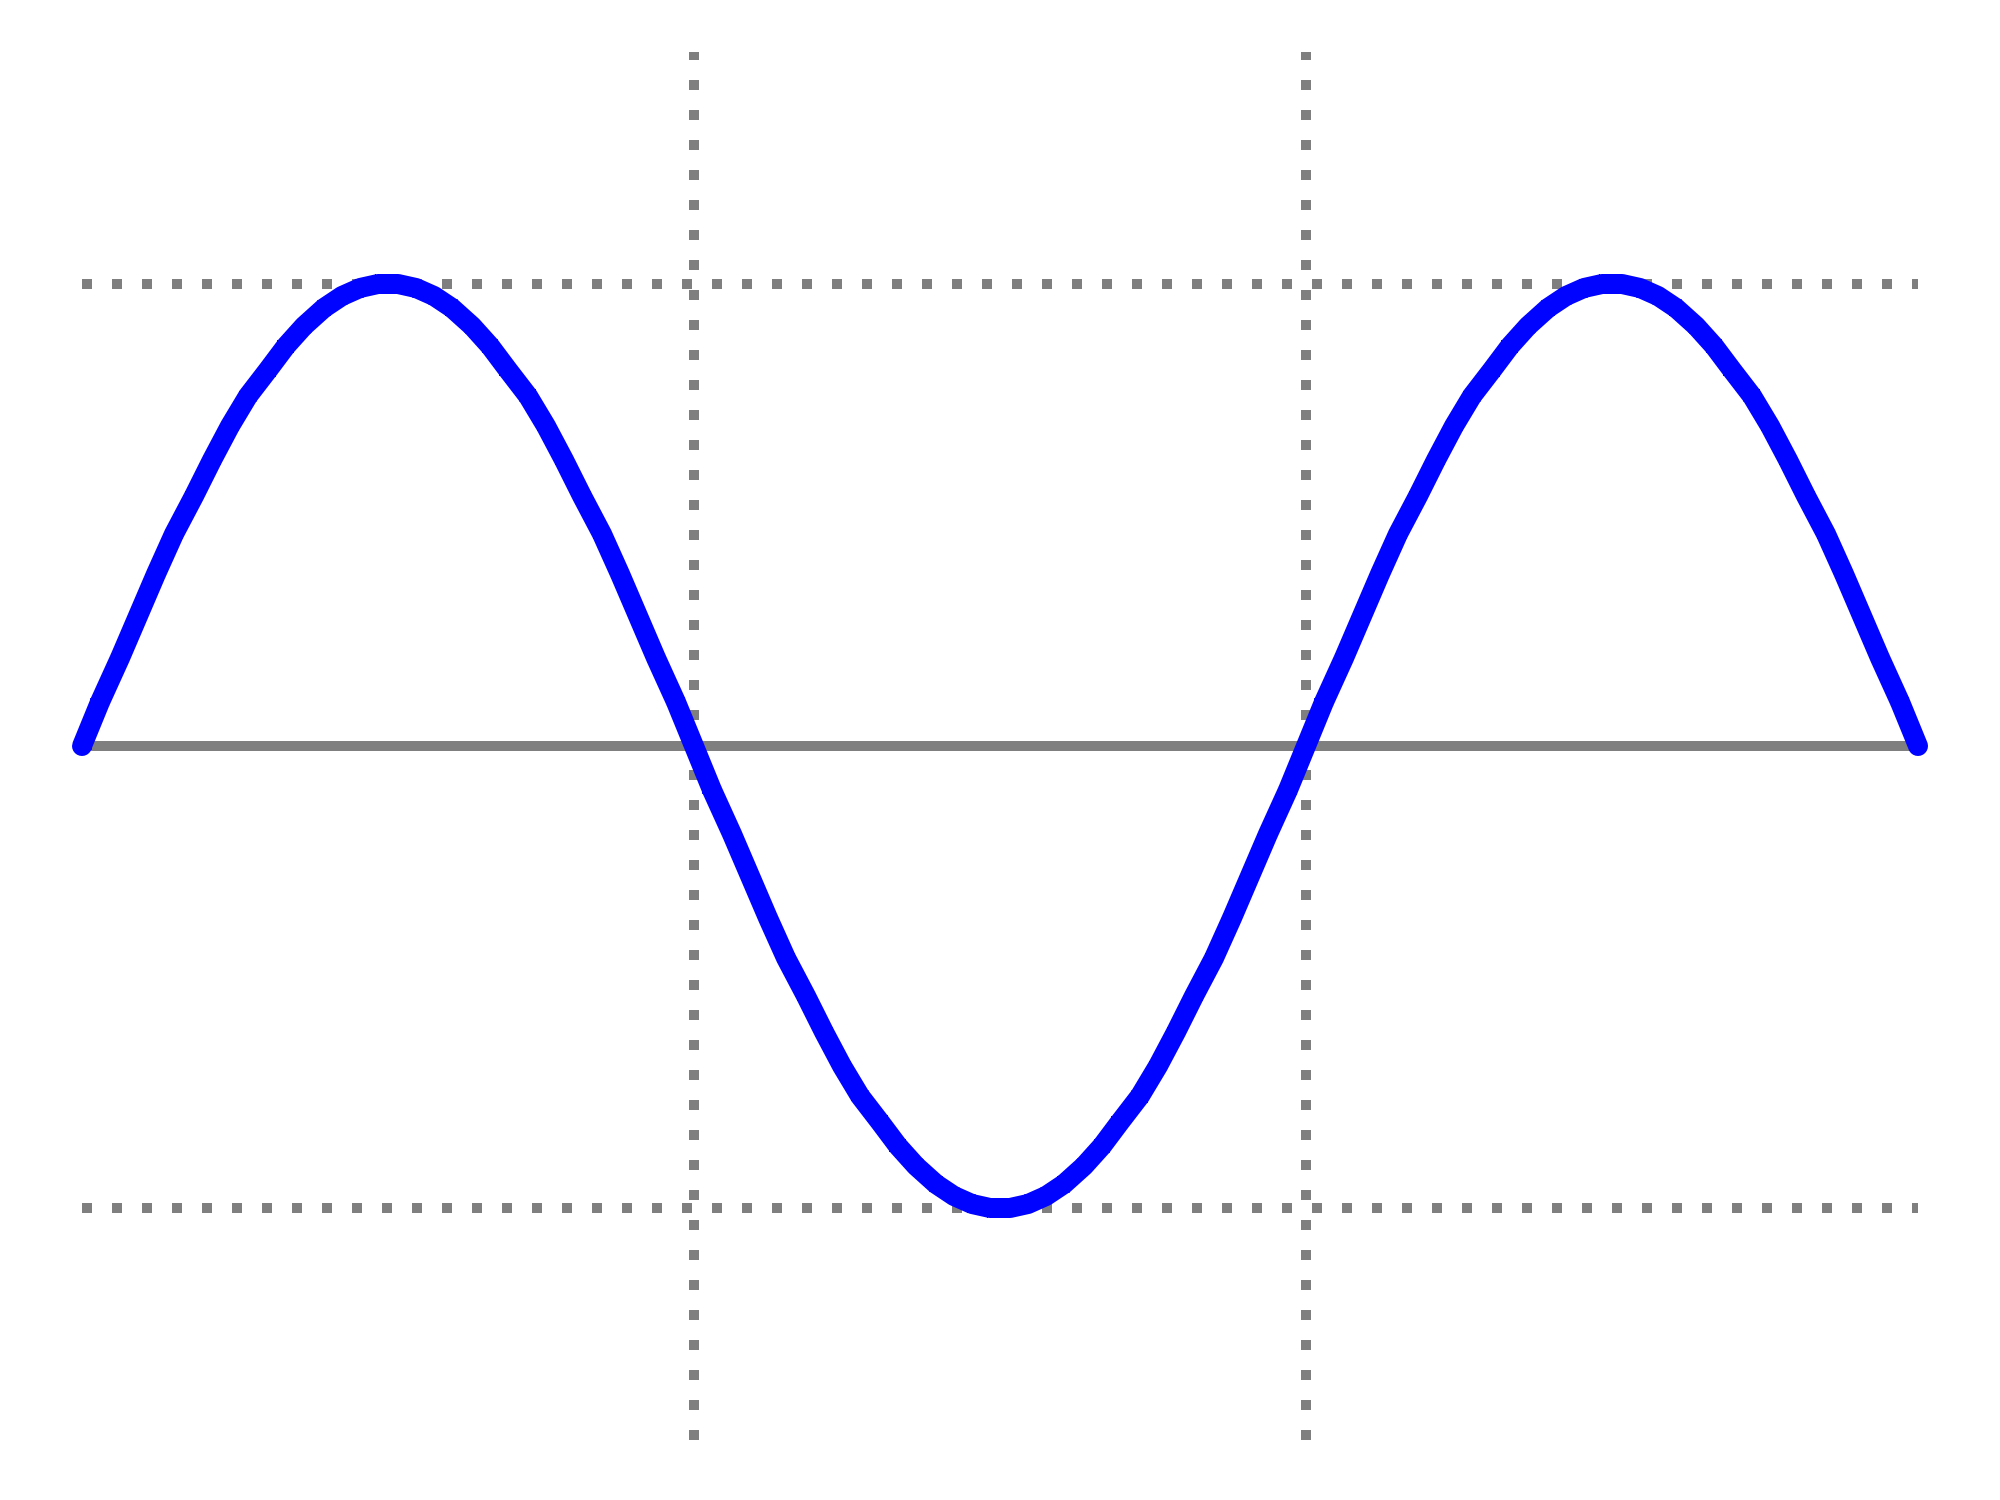
\includegraphics[width=2cm]{images/table_sine_wave.png} &
			$A\cdot\sin(t)$ &
			$\frac{2}{\pi} \approx 0.637$ &
			$\frac{\pi}{2\sqrt{2}} \approx 1.11$ &
			$\frac{1}{\sqrt{2}}\approx 0.707$ &
			$\sqrt{2}\approx 1.414$ &
			$0$ &
			$\frac{A^2}{2}$ &
			$\frac{A^2}{2}$ \\
			\hline	
			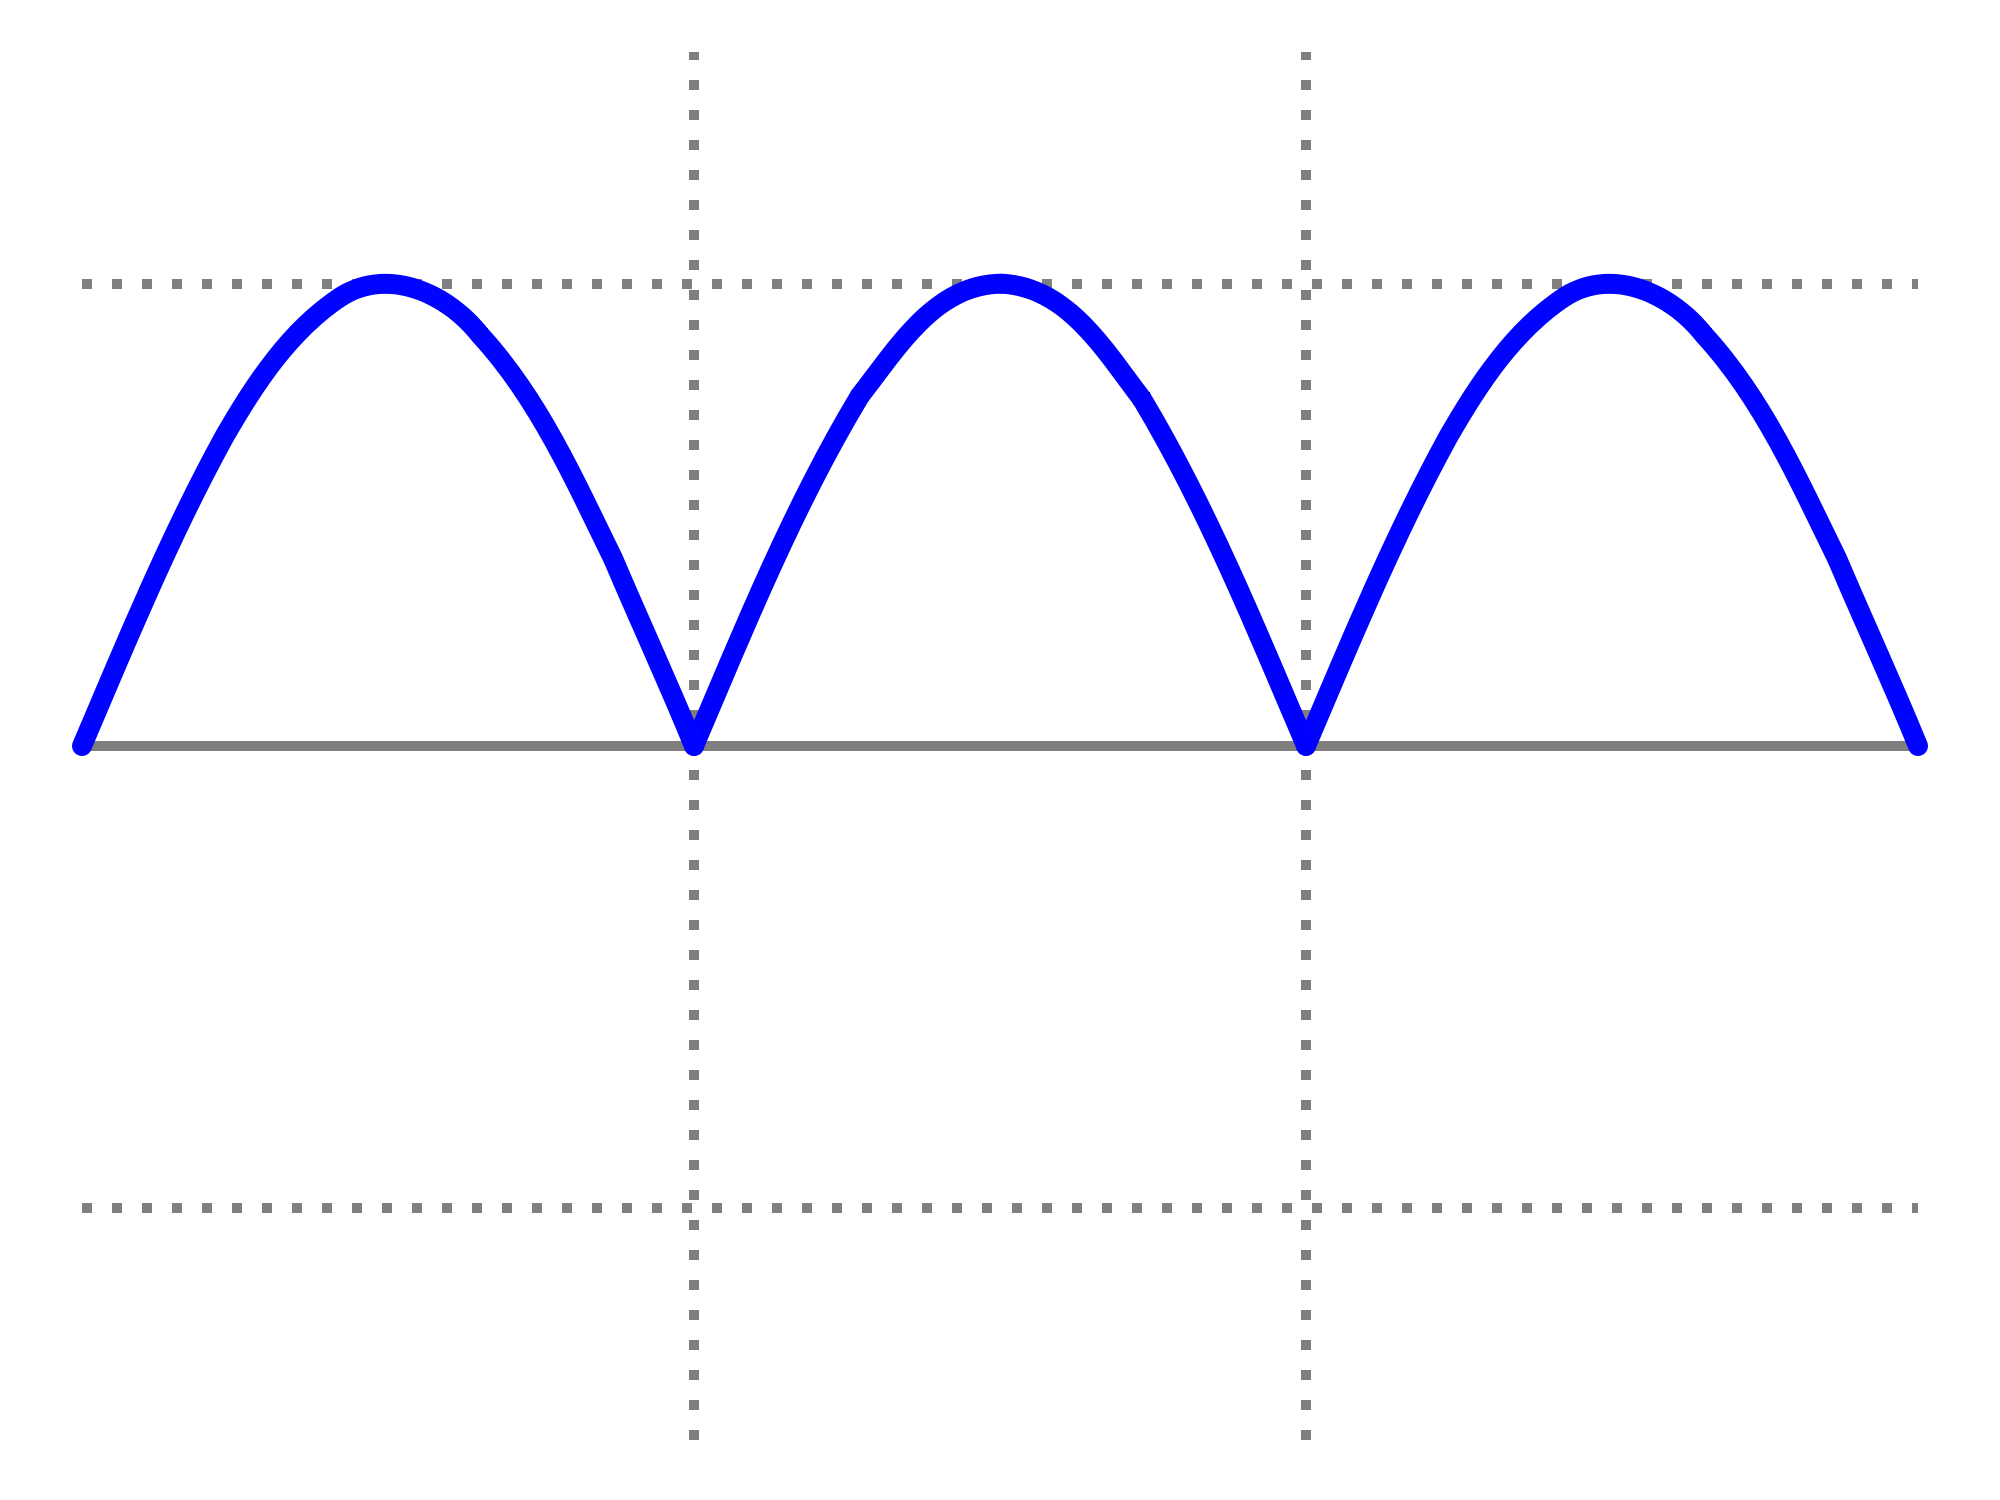
\includegraphics[width=2cm]{images/table_full-wave_rectified_sine.png} &
			$A\cdot|\sin(t)|$ &
			$\frac{2}{\pi} \approx 0.637$ &
			$\frac{\pi}{2\sqrt{2}} \approx 1.11$ &
			$\frac{1}{\sqrt{2}} \approx 0.707$ &
			$\sqrt{2} \approx 1.414$  &
			$\frac{2A}{\pi}$ & $\frac{A^2}{2}$ & $\frac{A^2}{2}-\frac{4A^2}{\pi^2}$
			\\
			\hline
			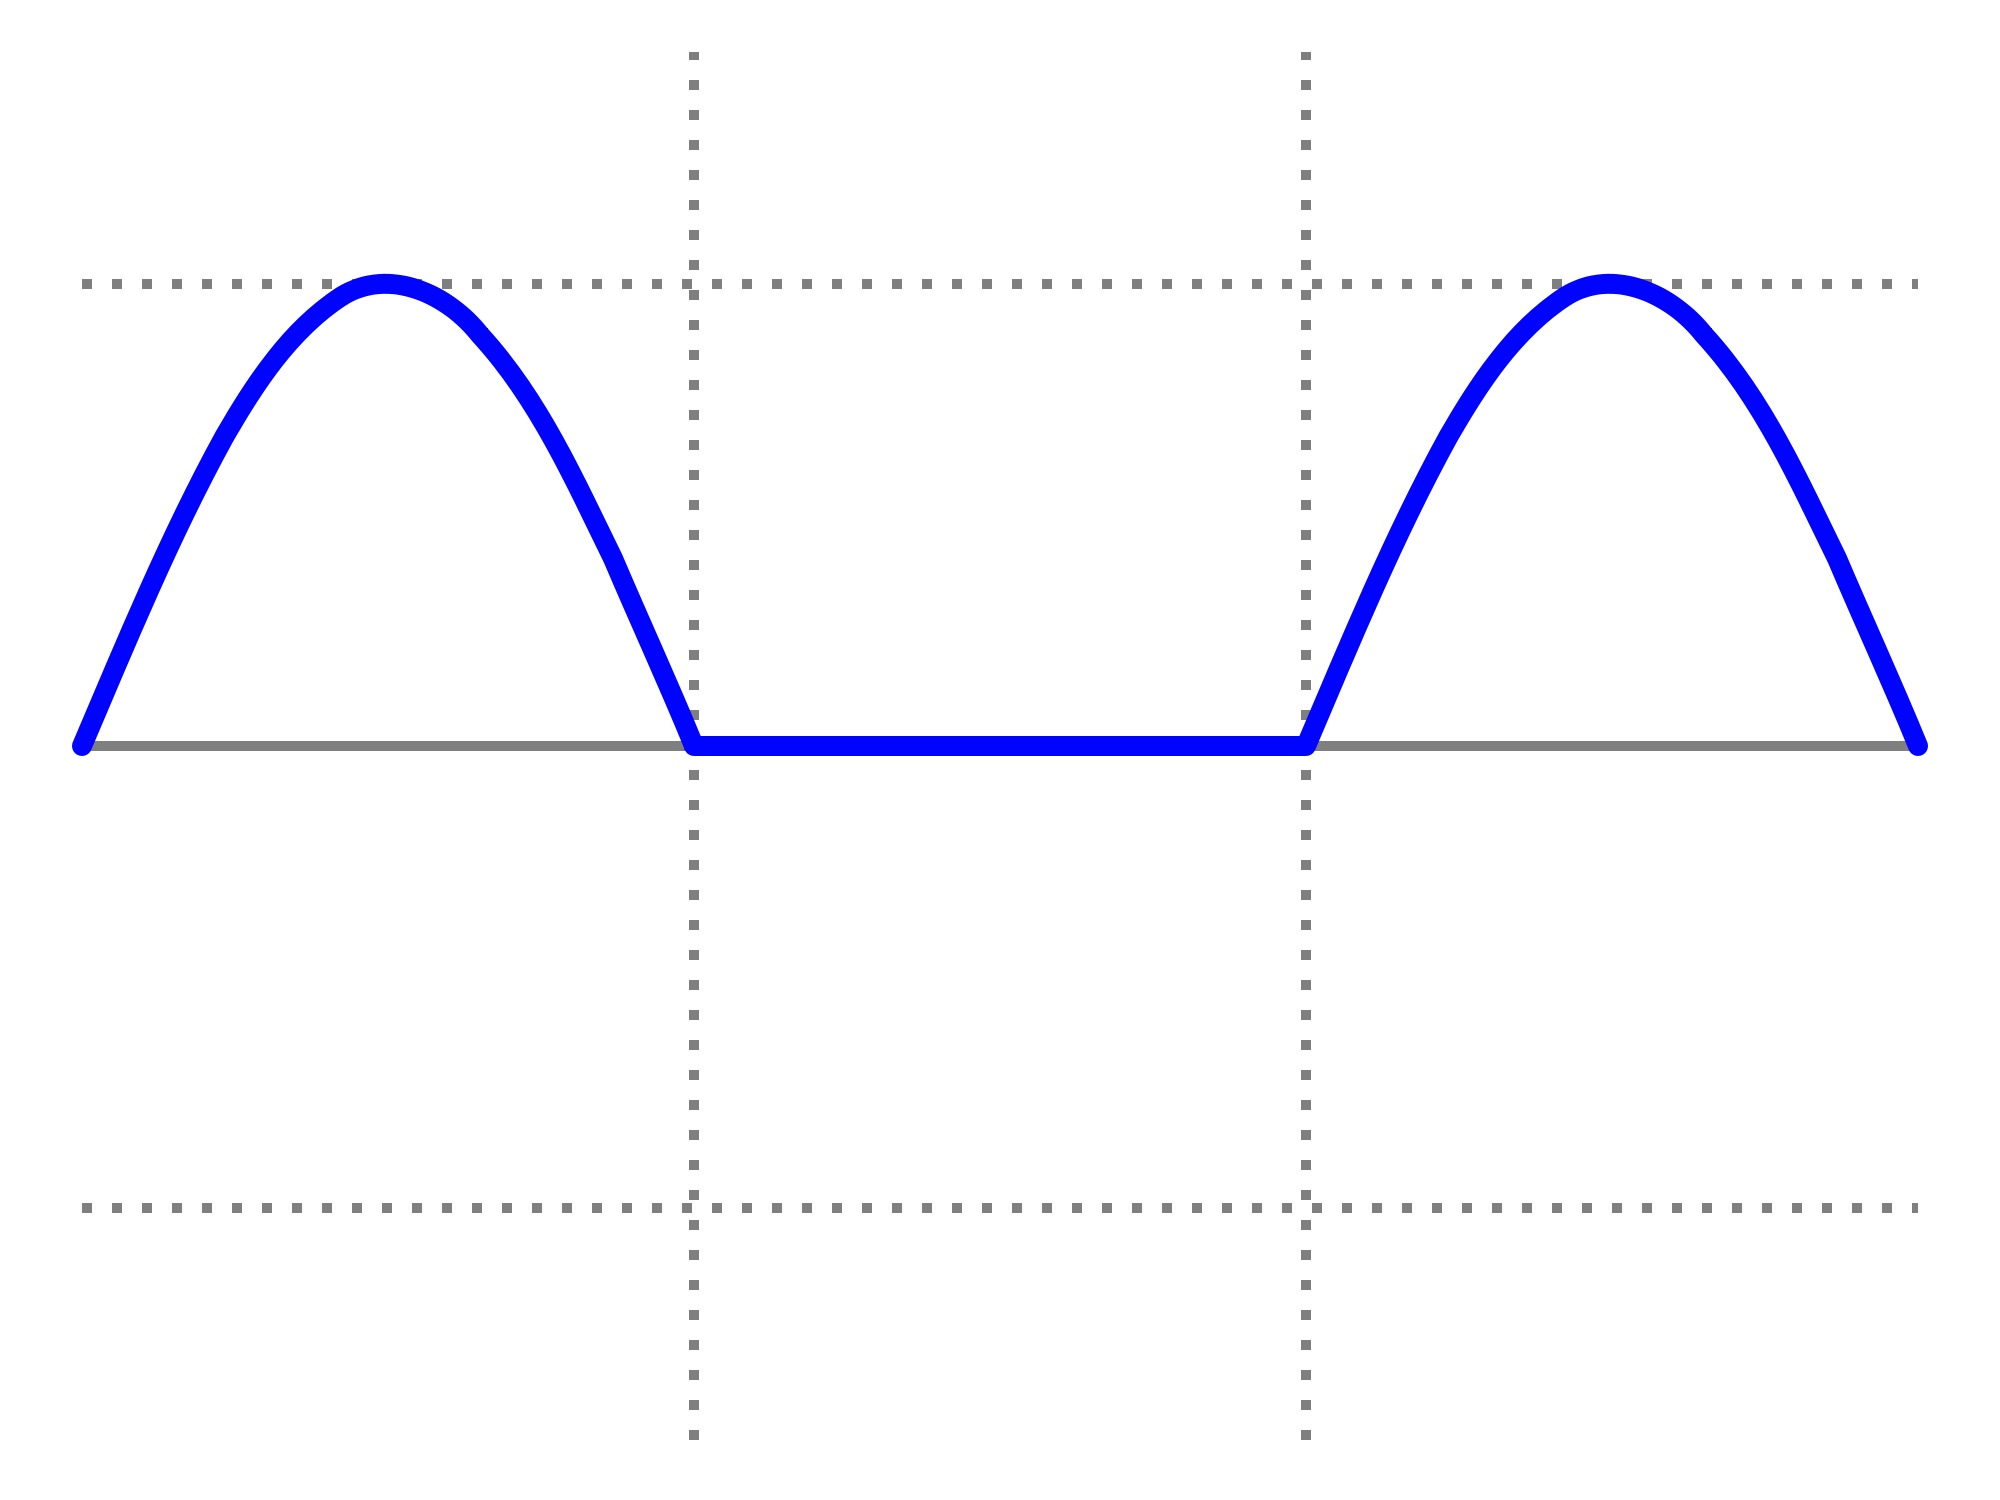
\includegraphics[width=2cm]{images/table_half-wave_rectified_sine.png} &
			$\begin{cases} A\cdot\sin (t) & 0<t<\pi  \\ 0 & \text{True}\end{cases}$ &
			$\frac{1}{\pi}\approx 0.318$ &
			$\frac{\pi}{2}\approx 1.571$ &
			$\frac{1}{2} = 0.5$	&
			2  &
			$\frac{A}{\pi}$ &
			$\frac{A^2}{4}$ & $\frac{A^2}{4}-\frac{A^2}{\pi^2}$
			\\
			\hline
			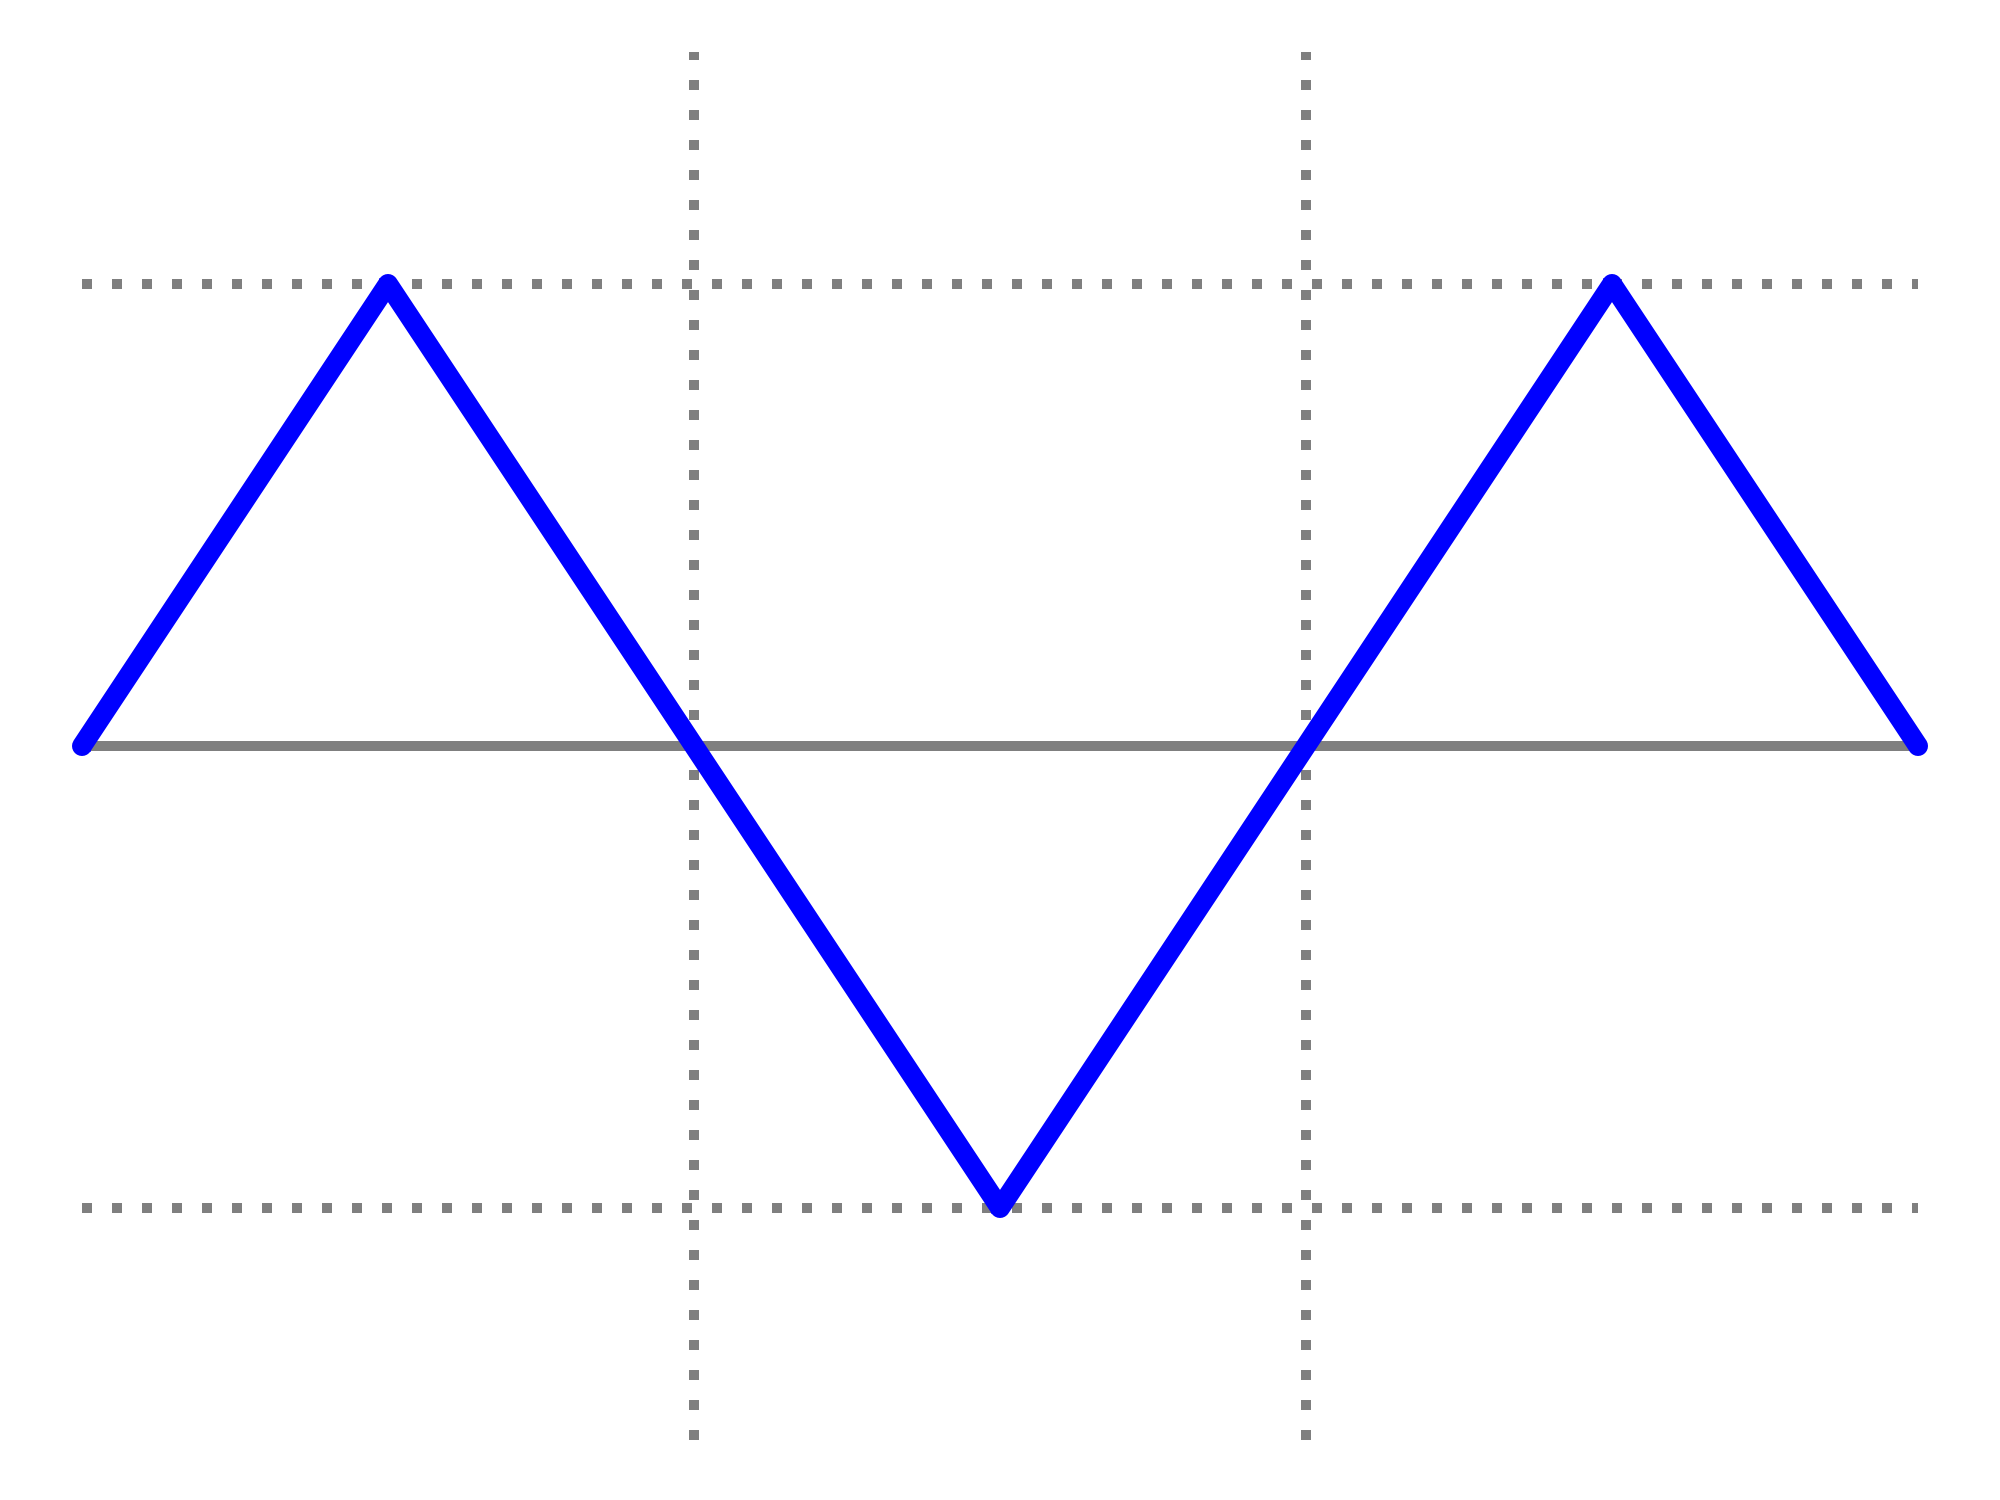
\includegraphics[width=2cm]{images/table_triangle_wave.png} &
			$A\cdot\Lambda(t)$ &
			$\frac{1}{2}= 0.5$ &
			$\frac{2}{\sqrt{3}}\approx 1.155$ &
			$\frac{1}{\sqrt{3}}
			\approx 0.557$ &
			$\sqrt{3} \approx 1.732$ &
			$0$ &
			$\frac{A^2}{3}$ &
			$\frac{A^2}{3}$ \\
			\hline	
			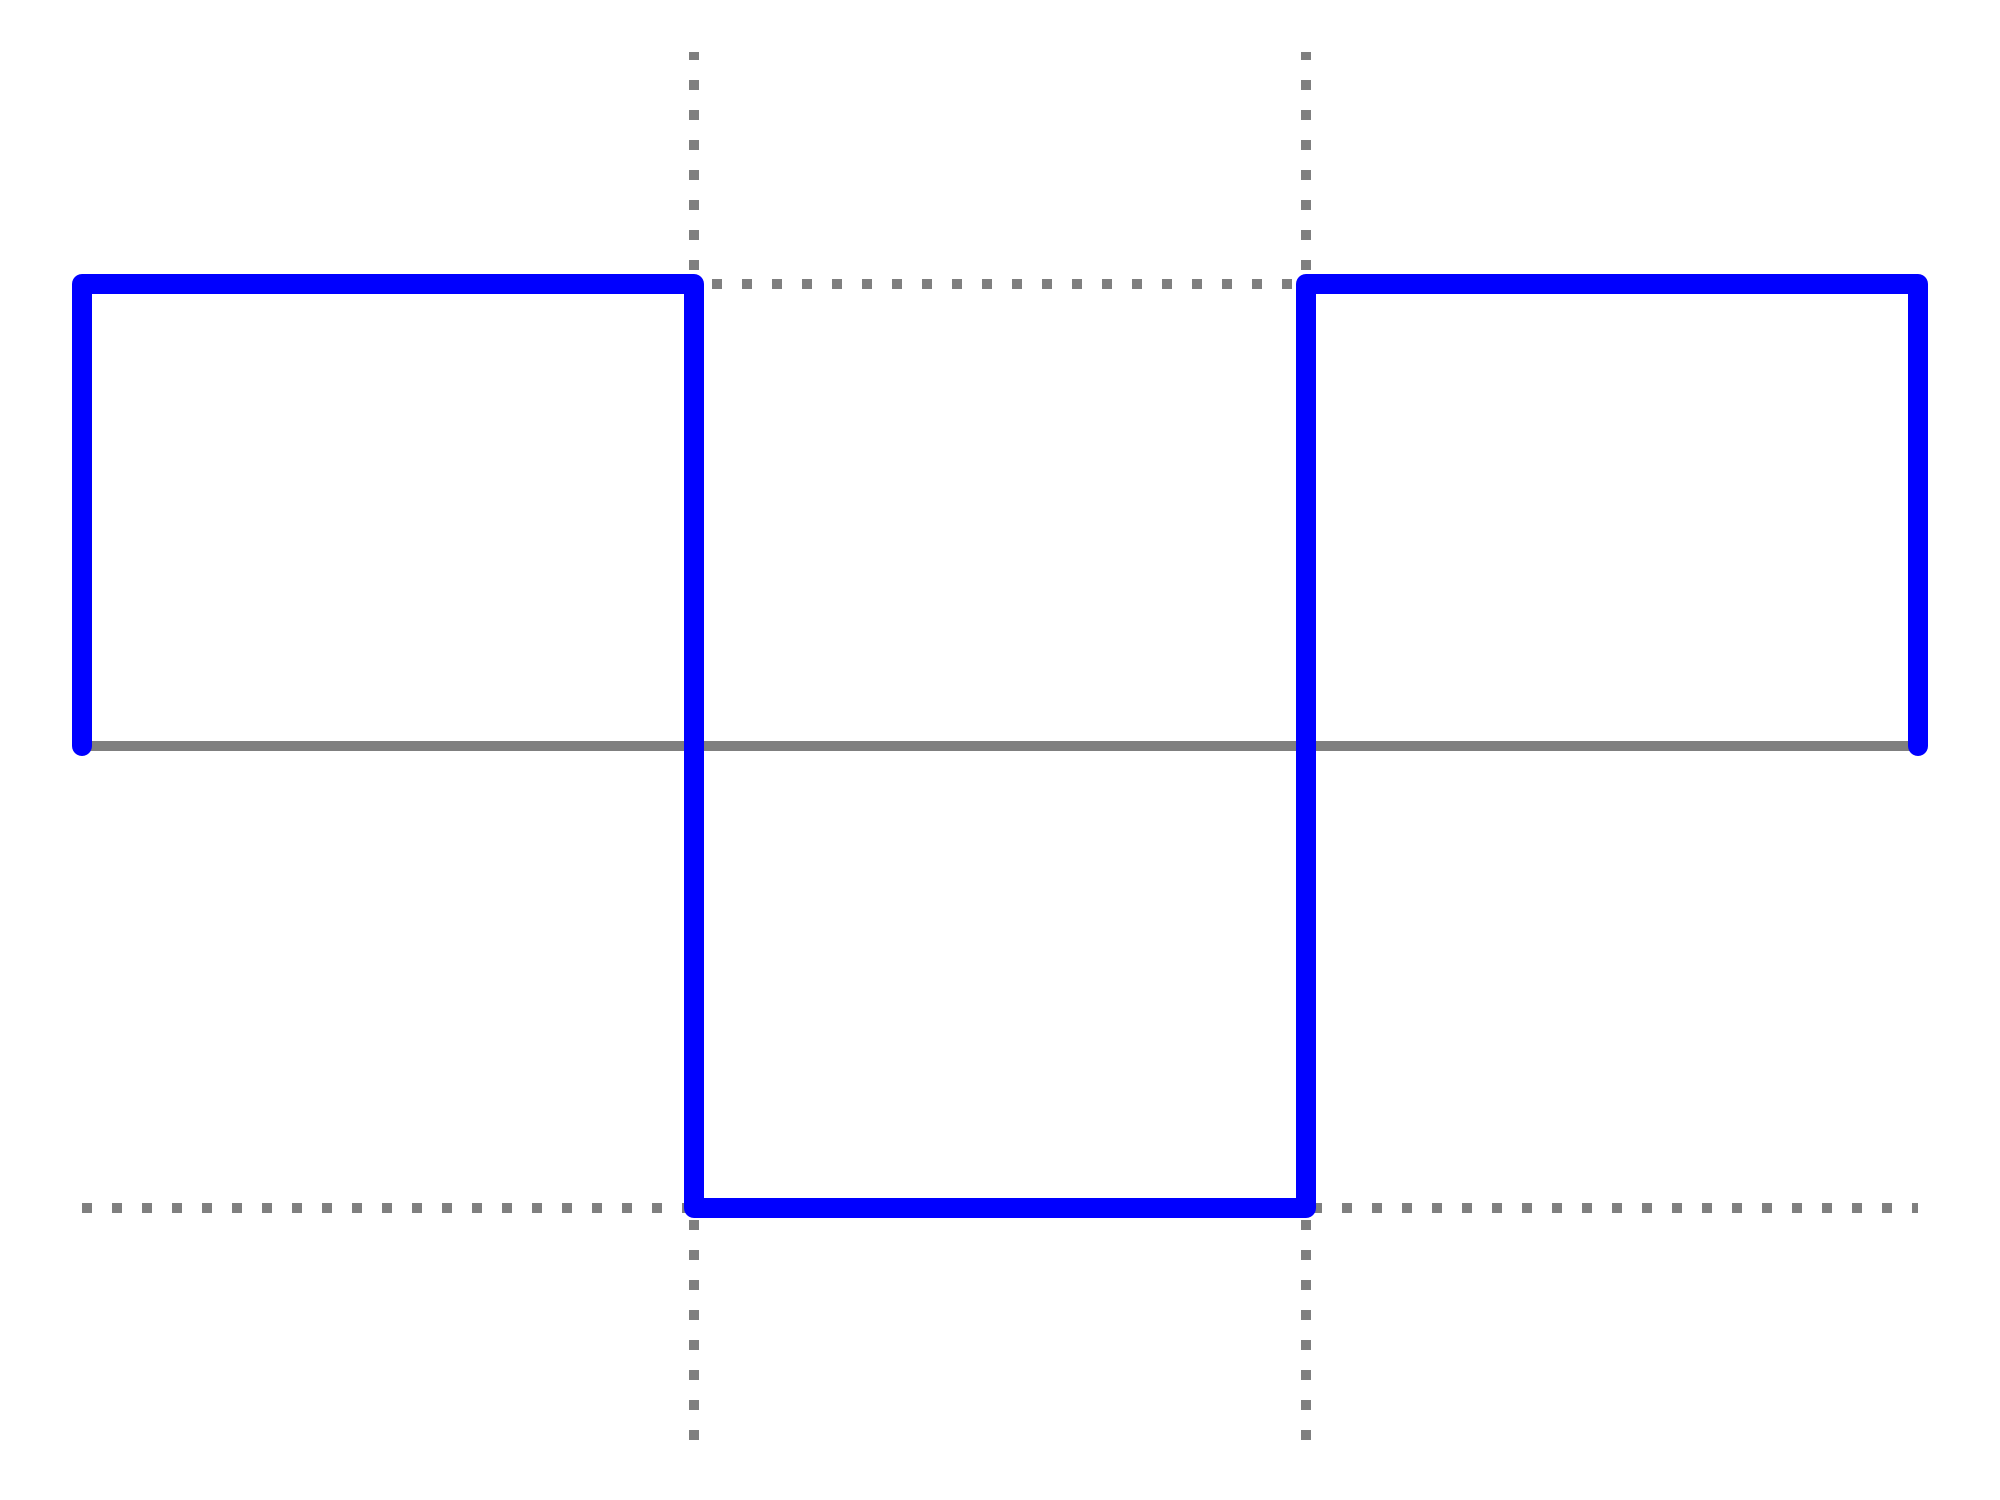
\includegraphics[width=2cm]{images/table_square_wave.png} &
			$\begin{cases} A & 0<x<t \\ 0 & \text{True}\end{cases}$ &
			$1$ &
			$1$ &
			$1$ &
			$1$ &
			$0$ &
			$A^2$ &
			$A^2$ \\
			\hline	
			DC&
			1&
			$1$ &
			$1$ &
			$1$ &
			$1$  &
			-&
			-&
			-\\
			\hline	
			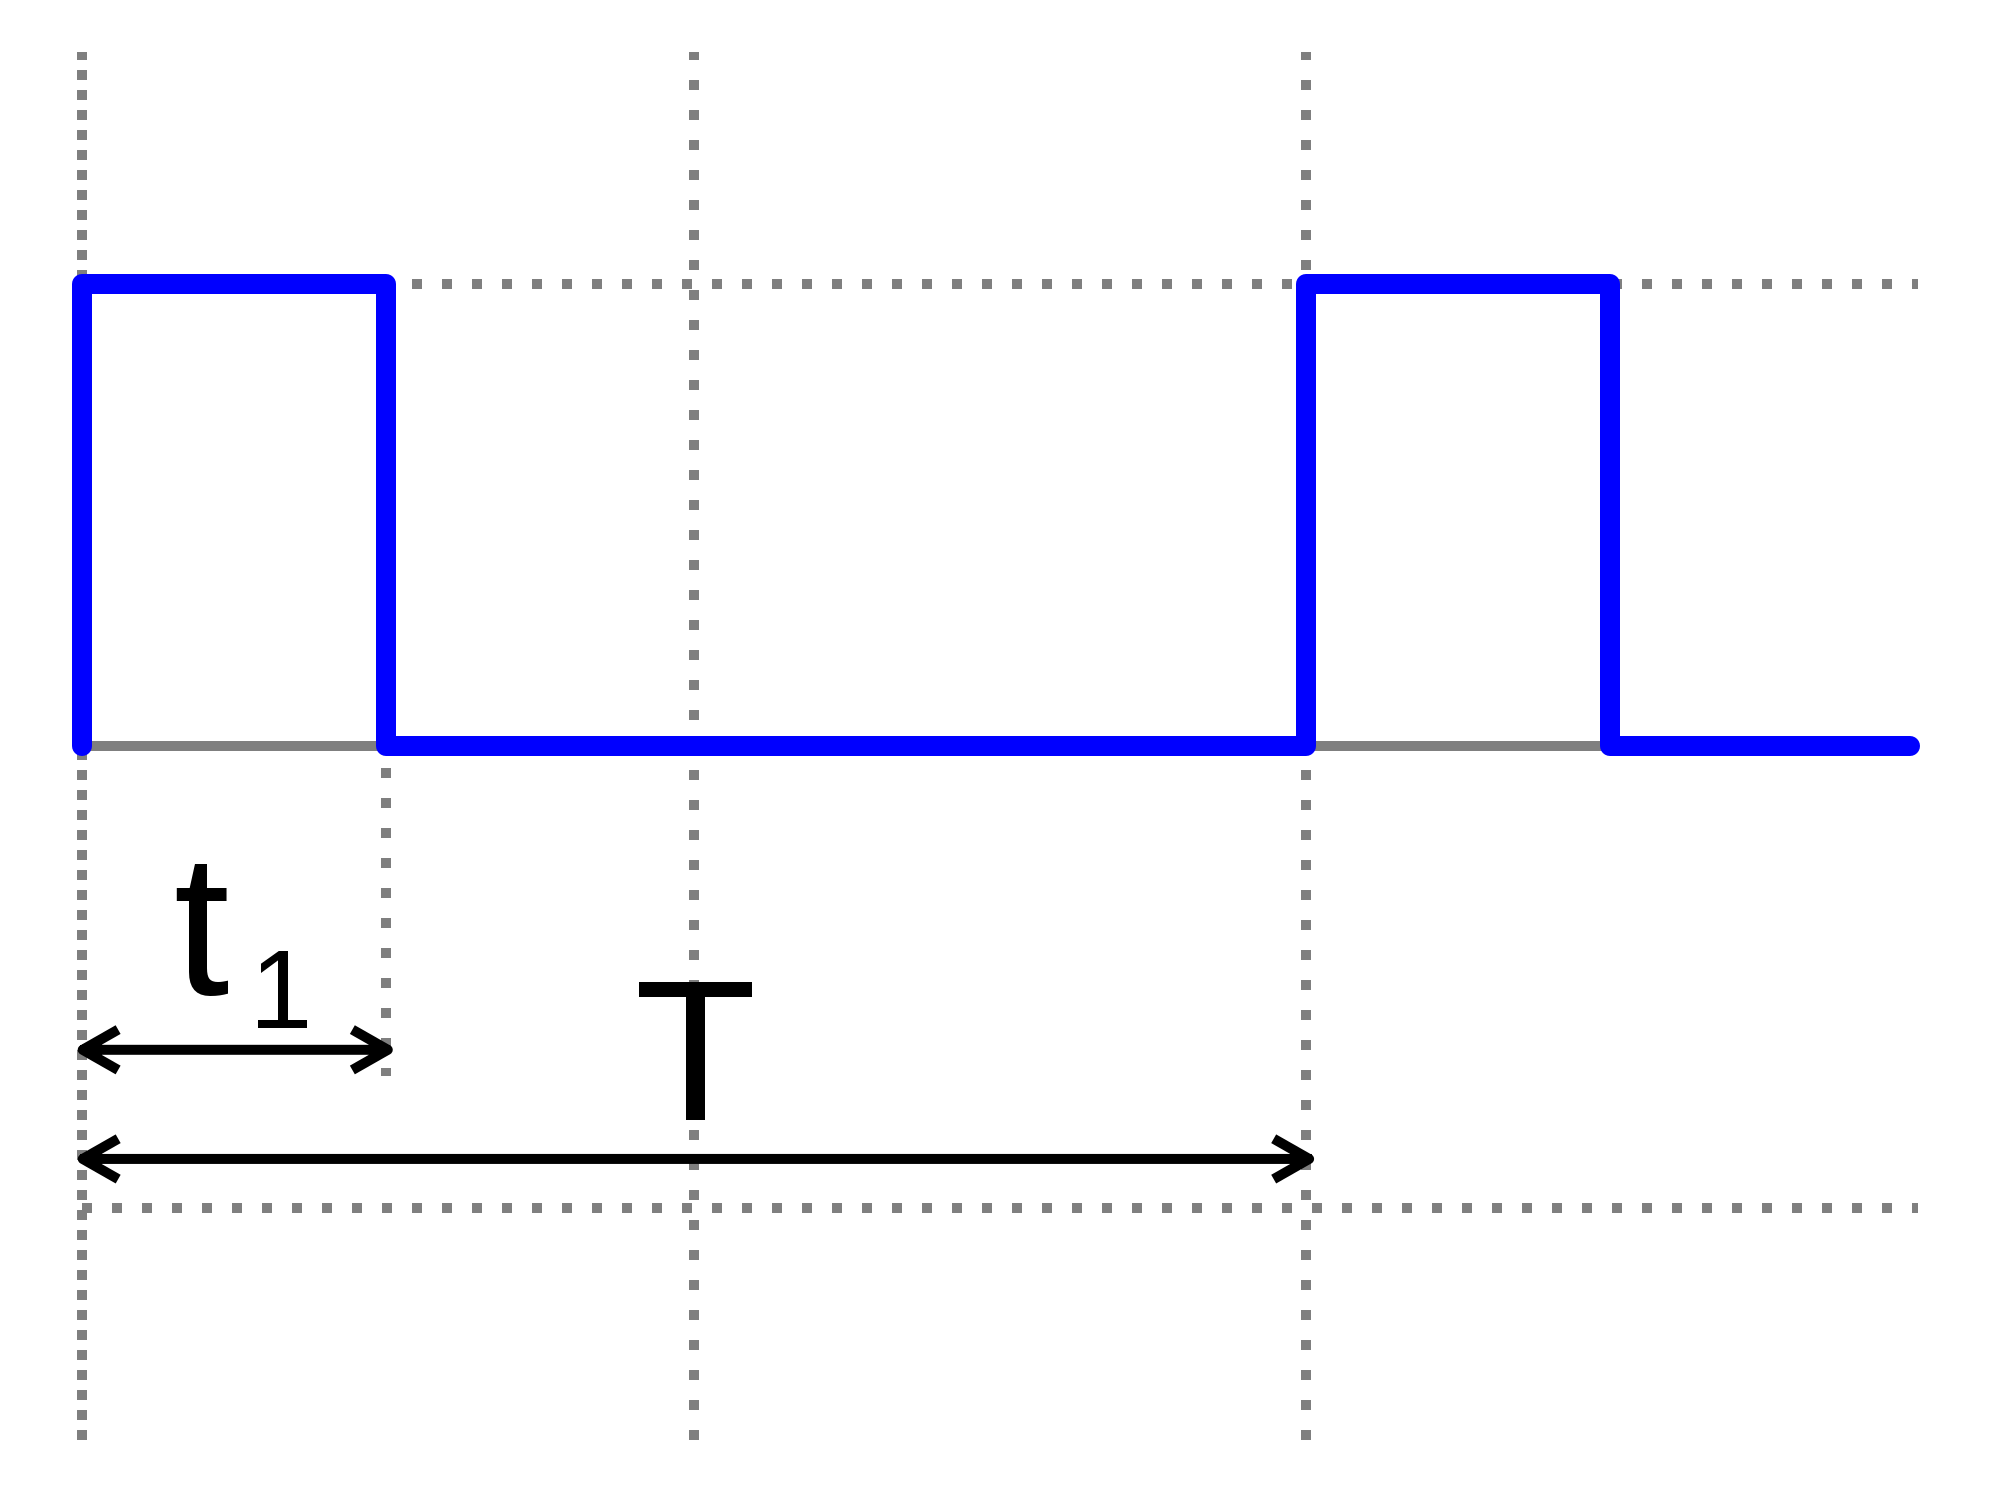
\includegraphics[width=2cm]{images/table_pulse_wide_wave.png} &
			&
			$\frac{t_1}{T}$ & $\sqrt{\frac{T}{t_1}}$ & $\sqrt{\frac{t_1}{T}}$ & $\sqrt{\frac{T}{t_1}}$ &
			$A\frac{t}{T}$ &
			$A^2\frac{t}{T}$ &
			$\frac{A^2t}{T}-\frac{A^2t^2}{T^2}$\\
			\hline
		\end{tabular}
\end{sidewaystable}
\clearpage
\newpage